\documentclass[conference]{IEEEtran}
\IEEEoverridecommandlockouts
% Funding-identification footnote is unused here; \IEEEoverridecommandlockouts
% is kept only because it is harmless to leave in and is required if a
% \thanks funding footnote is added later.

\usepackage{cite}
\usepackage{amsmath,amssymb,amsfonts}
\usepackage{algorithmic}
\usepackage{graphicx}
\usepackage{textcomp}
\usepackage{xcolor}
\usepackage{booktabs}
\def\BibTeX{{\rm B\kern-.05em{\sc i\kern-.025em b}\kern-.08em
    T\kern-.1667em\lower.7ex\hbox{E}\kern-.125emX}}
\begin{document}

\title{Multi-Agent Reinforcement Learning for Safety-Constrained Heterogeneous Automotive Over-the-Air Update Scheduling}

%%% NOTE FOR THE AUTHORS: VTC2027-Spring is NOT double-blind, unlike the
%%% AAMAS submission of this same work. Real author names, affiliations,
%%% and e-mail addresses are required. The placeholders below reflect the
%%% author and institution information used elsewhere in this project;
%%% please verify the department/city spelling and replace the e-mail
%%% placeholders with the authors' actual addresses before submission.

\author{\IEEEauthorblockN{Mahmudul Islam Mahin}
\IEEEauthorblockA{\textit{Computer Science and Engineering} \\
\textit{Islamic University of Technology (IUT)}\\
Boardbazar, Bangladesh \\
mahmudulislam@iut-dhaka.edu}
\and
\IEEEauthorblockN{Saadman Sakib}
\IEEEauthorblockA{\textit{Computer Science and Engineering} \\
\textit{Islamic University of Technology (IUT)}\\
Boardbazar, Bangladesh \\
saadmansakib@iut-dhaka.edu}
\and
\IEEEauthorblockN{Mohtasim Dipto}
\IEEEauthorblockA{\textit{Computer Science and Engineering} \\
\textit{Islamic University of Technology (IUT)}\\
Boardbazar, Bangladesh \\
mohtasimdipto@iut-dhaka.edu}
% \and
% \IEEEauthorblockN{4\textsuperscript{th} Given Name Surname}
% \IEEEauthorblockA{\textit{dept. name of organization (of Aff.)} \\
% \textit{name of organization (of Aff.)}\\
% City, Country \\
% email address or ORCID}
% \and
% \IEEEauthorblockN{5\textsuperscript{th} Given Name Surname}
% \IEEEauthorblockA{\textit{dept. name of organization (of Aff.)} \\
% \textit{name of organization (of Aff.)}\\
% City, Country \\
% email address or ORCID}
% \and
% \IEEEauthorblockN{6\textsuperscript{th} Given Name Surname}
% \IEEEauthorblockA{\textit{dept. name of organization (of Aff.)} \\
% \textit{name of organization (of Aff.)}\\
% City, Country \\
% email address or ORCID}
}

\maketitle
 
\begin{abstract}
Connected and autonomous vehicles rely on Over-the-Air (OTA) firmware updates to keep a heterogeneous fleet of Electronic Control Units (ECUs) -- engine, braking, infotainment, and others -- current and secure, but coordinating updates across such a fleet under a constrained wireless channel and a shared, hard memory-safety budget is a difficult scheduling problem, made harder by conflicting cost and risk profiles across ECU classes. We extend a single-agent OTA scheduling baseline into a multi-agent reinforcement learning (MARL) framework in which each ECU is an independent learning agent, coordinated through a Control-Barrier-Function-style safety shield and a Monte Carlo Shapley credit-assignment scheme. Using this environment, we compare a parameter-specialized architecture (FP3O) against fully shared, ECU-type-conditioned policies (IPPO, MAPPO) under a staged sequence of experiments that progressively increases functional heterogeneity between ECU types. In the process, we uncover and correct an observation-design confound -- a raw per-agent identifier that let a nominally shared policy covertly memorize per-agent behavior -- which had inflated the apparent advantage of the shared architecture by a wide margin. After correcting this and scaling to 5 seeds per algorithm, the shared, type-conditioned policies (IPPO and MAPPO, both 16.71 mean return, 95\% CI $\pm0.001$) are not only competitive with but dramatically more reliable than the specialized architecture (FP3O, 5.09 mean return, 95\% CI $\pm26.14$), whose headline mean is dominated by a single catastrophic-failure seed out of five ($-32.37$) rather than uniformly weaker performance. None of the pairwise comparisons reach conventional statistical significance at this sample size (IPPO vs.\ FP3O: $p=0.285$; IPPO vs.\ MAPPO: $p=0.079$), so this evidence is suggestive rather than confirmatory. The safety shield holds the fleet-wide memory-safety violation rate at 0\% throughout for all three algorithms. We discuss the implications of these findings -- both the confound and FP3O's seed instability -- for the design of MARL-based OTA update schedulers for connected vehicle fleets.
\end{abstract}
 
\begin{IEEEkeywords}
over-the-air updates, multi-agent reinforcement learning, connected and autonomous vehicles, electronic control units, safety-constrained learning, parameter sharing, intelligent transport systems
\end{IEEEkeywords}
 
\section{Introduction}
 
Modern connected and autonomous vehicles (CAVs) are distributed computing platforms built from dozens of Electronic Control Units (ECUs) governing engine timing, braking, infotainment, and driver-assistance functions. Like any networked software system, these ECUs require periodic firmware updates to patch vulnerabilities, fix defects, and add functionality, and Over-the-Air (OTA) delivery has become the industry standard because it avoids costly dealership recalls and reduces update latency across a fleet.
 
The engineering difficulty of fleet-wide OTA updates is easy to underestimate. ECUs differ substantially in their tolerance for risk and in their available flash-memory budget: a braking-system ECU cannot be updated the same way as an infotainment unit, both because a failed brake-ECU update is a safety hazard and because the two devices typically have very different memory constraints. At the same time, updates are usually delivered over a shared, congested, and unreliable wireless channel, so updating multiple ECUs concurrently is a scheduling problem -- which firmware blocks to send first, using which update technique, to which ECU -- subject to a fleet-wide memory-safety budget that must never be exceeded.
 
Because this is a sequential decision problem under uncertainty, reinforcement learning (RL) is a natural fit. ReLES-OTA \cite{b1} demonstrated that a single RL agent can schedule OTA update operations for one vehicle more efficiently than heuristic baselines by formulating the problem as a Markov Decision Process (MDP). That formulation, however, treats the vehicle as a single decision point responsible for all of its ECUs at once, which becomes an increasingly unrealistic abstraction as fleets scale and as ECUs grow more heterogeneous.
 
We reframe fleet-wide OTA scheduling as a cooperative multi-agent reinforcement learning (MARL) problem, in which each ECU is its own agent, coordinated through a shared safety constraint and a fairly attributed team reward. This reframing surfaces an architectural design question of direct practical relevance to CAV platforms: when ECUs have systematically different roles and conflicting cost profiles, does the on-board (or fleet-management) scheduler need a dedicated, specialized policy per ECU type, or does a single shared policy -- conditioned only on ECU type -- suffice? The former is more expensive to train, certify, and maintain as new ECU classes are introduced to a vehicle platform; the latter scales more gracefully but risks losing accuracy if agents' incentives genuinely conflict. Architectures such as FP3O \cite{b2} build in explicit per-type specialization to resolve exactly this kind of conflict, while an influential empirical study \cite{b3} argues that fully shared policies (IPPO, MAPPO, built on PPO \cite{b4}) are competitive in cooperative multi-agent games because they pool experience across all agents -- but this claim has mostly been tested on largely homogeneous benchmarks, not under the hard safety constraints and structurally conflicting incentives that automotive ECU heterogeneity introduces.
 
Our contributions are: (1) a safety-constrained, Shapley-credited multi-agent OTA scheduling environment for heterogeneous CAV fleets, extending \cite{b1} to the multi-agent case; (2) a numerically stabilized large-scale PPO-family training recipe for this environment; (3) a staged, confound-aware empirical comparison of a specialized MARL architecture against fully shared, type-conditioned policies under genuine ECU-type conflict; and (4) the identification and correction of an agent-identity observation-design confound that had been silently favoring the shared-policy architecture, with implications for MARL-based scheduler design beyond this specific application.
 
\section{Related Work}
 
\subsection{OTA Update Scheduling for Connected Vehicles}
Automotive OTA scheduling has traditionally relied on heuristic and combinatorial schedulers, which generalize poorly as ECU diversity and network variability grow. ReLES-OTA \cite{b1} reframes single-vehicle OTA scheduling as a sequential codec-construction MDP and solves it with single-agent deep RL, reducing data-payload size and memory overhead relative to random- and sequential-order baselines. This single-agent formulation implicitly treats a vehicle's ECUs as one decision point, which is the gap this work addresses by lifting the problem into a multi-agent setting where each ECU has independently varying backlog, cost structure, and safety requirements.
 
\subsection{Cooperative Multi-Agent Reinforcement Learning}
Cooperative MARL methods generally follow a Centralized-Training-Decentralized-Execution (CTDE) paradigm. Value-based approaches such as VDN \cite{b12} and QMIX \cite{b13} factorize a joint value function into per-agent components, while actor-critic approaches such as MADDPG \cite{b10} and COMA \cite{b11} augment each agent's critic with joint information during training. Building on PPO \cite{b4}, an empirical study \cite{b3} showed that fully shared IPPO/MAPPO policies are competitive with, and often exceed, more complex architectures on cooperative benchmarks, attributing this to full sample reuse across agents. FP3O \cite{b2} instead shares a common backbone but routes it into per-agent-type specialized heads, aiming to combine sample efficiency with the flexibility needed to represent conflicting per-type behavior; we use FP3O as our specialized-architecture baseline. Terry et al.\ \cite{b14} caution that parameter-sharing benefits depend on agent homogeneity and, critically, on how agent identity is encoded in the observation space -- a caution our confound finding (Section~V) confirms concretely.
 
\subsection{Safety-Constrained Learning for Vehicular Systems}
We adopt a rule-based safety filter inspired by Control Barrier Functions (CBFs) \cite{b15}, which guarantee that a system's state remains within a safe set by overriding unsafe actions. CBF-based safety shields have recently been used in multi-agent driving policies: RSR-RSMARL \cite{b16} uses a CBF-based shield for safe sim-to-real transfer of a multi-agent driving policy on 1/10th-scale hardware, and MAPPO-PIS \cite{b17} incorporates a safety-enhancement module into a shared-policy MARL pipeline for cooperative decision-making among connected vehicles at merging areas. We follow the same design philosophy: an external, rule-based filter rather than reward shaping alone, since the latter offers no hard guarantee during the high-variance early stages of training.
 
\subsection{Credit Assignment}
Splitting a shared team reward fairly among agents is addressed by counterfactual baselines \cite{b11} and, more generally, by the game-theoretic Shapley value \cite{b18}, which allocates a coalition's payoff based on each member's average marginal contribution across all possible join orders. We use a Monte Carlo approximation of the Shapley value for tractability at our fleet sizes.
 
\section{Environment and Methodology}
 
\subsection{Single-Agent Baseline}
We first reproduce the ReLES-OTA \cite{b1} cost model in a single-agent Gymnasium \cite{b8} environment, where an agent selects a firmware block and an update operation at each step and receives a reward combining encoding cost, a stochastic truncated-Gaussian transmission cost, and memory overhead. A PPO \cite{b4} policy trained on this environment reaches a mean return of approximately $-18$, matching the trend of the original single-agent result and validating our reimplementation before scaling to multiple agents.
 
\subsection{Multi-Agent Environment}
We extend the environment to a PettingZoo Parallel-API \cite{b9} setting with $N$ concurrent ECU agents, each with an independent firmware backlog and a per-step action mask that disables already-updated blocks. Three components support the safety- and fairness-critical aspects of the fleet setting.
 
\textit{Death masking}: agents that finish their backlog before the episode ends receive a fixed zero-vector observation (preserving only their type identity) rather than being removed, keeping tensor shapes constant for the centralized critic, following the convention used in recent multi-agent driving work \cite{b17}.
 
\textit{Safety shield}: a rule-based filter inspired by CBFs \cite{b15} intercepts every proposed joint action and overrides or blocks any action that would push cumulative fleet memory usage above 85\% of budget, in the spirit of the CBF-based per-agent shields used in \cite{b16}. This guarantees safety independent of policy quality, which matters most during early, near-random exploration.
 
\textit{Monte Carlo Shapley credit assignment}: because the environment returns a single team reward, we approximate each agent's Shapley value \cite{b18} by sampling random agent orderings and averaging each agent's marginal contribution across samples, avoiding the bias a naive equal-split reward would introduce once ECU types carry different operation costs.
 
\subsection{Policy Architectures}
All architectures follow CTDE. \textbf{IPPO} trains one shared policy network across all agents with no architectural type distinction. \textbf{MAPPO} shares actor parameters but pairs them with a fully centralized critic conditioned on the joint observation. \textbf{FP3O} \cite{b2} shares a common MLP backbone (256$\to$256$\to$128) but routes it into per-ECU-type specialized action and position heads. FP3O operationalizes the hypothesis that specialization is necessary; IPPO/MAPPO operationalize the hypothesis that type-conditioned sharing suffices.
 
\subsection{Training Stability}
At full scale (2M timesteps), extreme PPO probability ratios combined with rare, large safety-shield crash penalties caused Adam's \cite{b19} second-moment estimate to overflow, producing NaN logits. We resolved this via (i) tightening the logit clamp to $[-10,10]$, (ii) a target-KL early-stopping criterion, (iii) replacing a custom value normalizer with Stable-Baselines3's \cite{b20} \texttt{VecNormalize}, and (iv) capping the maximum crash penalty. Training was stable across all seeds and architectures thereafter.
 
\subsection{Staged Heterogeneity Design}
We introduce ECU-type heterogeneity in four stages so that any performance gap can be attributed to a specific cause: (S1) a \textit{homogeneous} fleet where type labels do not affect reward, cost, or dynamics; (S2) a \textit{uniform cost-multiplier} stage applying a per-type scalar cost multiplier; (S3) an \textit{operation-specific multiplier} stage where safety-critical types (engine, braking) are structurally incentivized toward a costlier, more reliable Multi-Base (MB) update operation while other types remain incentivized toward a cheap Copy operation, creating a genuine conflict in optimal per-type behavior; and (S4) a \textit{corrected re-comparison} of S3 after removing an observation-design confound discovered in S3.
 
\section{Experimental Setup}
All headline experiments use 4 ECU agents, 16 firmware blocks per agent, and a 2,000,897-timestep training horizon per seed, with the safety-shield threshold fixed at 85\% of the memory budget. All architectures use the training-stability configuration of Section~III-D. Results are averaged over 5 random seeds per algorithm (up from an earlier 2-seed pass), which we identify as still short of full statistical power in Section~VI.
 
\section{Results}
 
\textbf{S1 -- Homogeneous fleet.} With no genuine heterogeneity, IPPO/MAPPO outperform FP3O (approx.\ 12.85 vs.\ 11.44 mean return), consistent with \cite{b3}: FP3O's specialized heads each receive only a fraction of the fleet's gradient updates, offering no benefit when there is nothing to specialize for.
 
\textbf{S2 -- Uniform cost multiplier.} A purely quantitative per-type cost multiplier does not change the \textit{ordinal} preference of update operations -- every type still prefers the cheapest Copy operation -- so this stage is inconclusive.
 
\textbf{S3 -- Genuine conflict and the agent-identity confound.} Once operation-specific multipliers create a genuine conflict, IPPO continues to dominate FP3O by a wide margin (16.71 vs.\ 8.68 mean return), which at face value would strongly favor shared policies. Investigating this gap, we found that each agent's observation included a raw per-agent one-hot identifier. Because agent-to-type assignment was fixed for a training run, this identifier let IPPO's nominally shared policy learn a distinct sub-policy per agent index -- a hidden, per-agent lookup table -- while still benefiting from four-fold pooled gradient updates. IPPO therefore held an unfair sample-efficiency advantage created by the observation design, not by the shared-parameter architecture itself, directly confirming the caution raised in \cite{b14} in a concrete numerical instance relevant to fleet-scheduler design.
 
\textbf{S4 -- Fair re-comparison, scaled to 5 seeds.} We replaced the raw agent identifier with a semantic, non-identifying \texttt{ecu\_type} one-hot vector and re-ran all three algorithms under the corrected observation space at 5 seeds each (2,000,897 timesteps/seed), superseding an earlier 2-seed pass in which MAPPO had not yet been retrained under the corrected observation space. Table~\ref{tab:leaderboard} reports this authoritative comparison. Type-conditioned IPPO and MAPPO are statistically indistinguishable from one another and extremely stable across seeds (16.71 vs.\ 16.71, 95\% CI half-width $\approx 0.001$ for both), indicating that full parameter sharing is sufficient in this environment regardless of whether a centralized critic is added on top of it. FP3O, by contrast, is seed-unstable: per-seed returns were $\{15.09, 15.18, 10.85, 16.71, -32.37\}$ -- four of five seeds cluster within a few points of the IPPO/MAPPO range (mean $14.46$, $sd=2.52$ excluding the outlier), but one seed collapsed to $-32.37$, which alone drags FP3O's reported mean down to $5.09$ and inflates its 95\% CI to $\pm26.14$ (Fig.~\ref{fig:comparison}). This is a new finding beyond the original agent-identity confound: FP3O's specialized-head architecture is not only less sample-efficient than a shared policy here, it is also less \textit{reliable} across random initializations, which matters directly for certifying a scheduler intended for on-vehicle or fleet-management deployment.
 
Welch's $t$-tests (unequal variance) computed directly from the per-seed return arrays show that none of the pairwise comparisons reach conventional significance at $n=5$ per arm: IPPO vs.\ FP3O gives $t(4.00)=1.23$, $p=0.285$, Cohen's $d=0.78$ (Hedges' $g=0.71$); IPPO vs.\ MAPPO gives $t(7.99)=2.01$, $p=0.079$, Cohen's $d=1.27$ (Hedges' $g=1.15$) -- a large effect size driven by the near-zero within-group variance rather than a large mean gap; and excluding FP3O's single outlier seed ($n=4$) raises its mean to $14.46$ and narrows the gap to $t(3.00)=1.79$, $p=0.171$, reinforcing that FP3O's headline number is dominated by one failed seed rather than a systematically worse policy. All three algorithms hold safety-shield activation at 0.0 (Fig.~\ref{fig:payload}), confirming the shield prevents unsafe fleet-memory states without needing to intervene once training converges, but mean payload cost for every algorithm remains far above the project's 5{,}000-byte deployment target, and is highest for FP3O (45{,}244.7 vs.\ $\approx$38{,}335 for IPPO/MAPPO).
 
\begin{table}[htbp]
\caption{Authoritative, \texttt{ecu\_type}-conditioned leaderboard (4 agents, 16 blocks/agent, 5 seeds, 2,000,897 timesteps/seed).}
\begin{center}
\begin{tabular}{lccccc}
\toprule
\textbf{Algo.} & \textbf{Return} & \textbf{95\% CI} & \boldmath{$p$} \textbf{vs.\ IPPO} & \textbf{Payload (B)} & \textbf{Shield} \\
\midrule
IPPO  & \textbf{16.71} & 0.001  & --      & 38{,}335.2 & 0.0 \\
MAPPO & 16.71          & 0.001  & 0.0791  & 38{,}336.5 & 0.0 \\
FP3O  & 5.09           & 26.14  & 0.2846  & 45{,}244.7 & 0.0 \\
\bottomrule
\end{tabular}
\label{tab:leaderboard}
\end{center}
\end{table}
 
\begin{figure}[htbp]
\centering
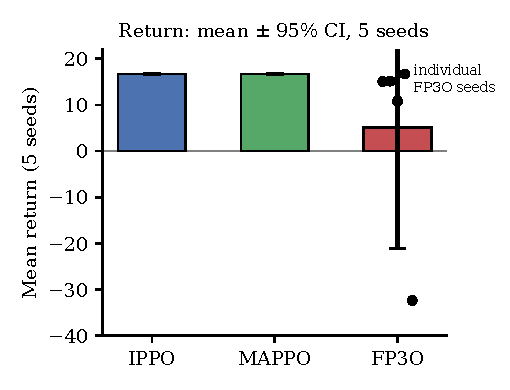
\includegraphics[width=0.85\linewidth]{figures/algo_comparison_3way.pdf}
\caption{Mean return with 95\% CI for IPPO, MAPPO, and FP3O (5 seeds each), reconstructed from the project's per-seed result files. Black points show FP3O's individual per-seed returns, isolating the single outlier seed ($-32.37$) responsible for its wide interval and low mean.}
\label{fig:comparison}
\end{figure}
 
\begin{figure}[htbp]
\centering
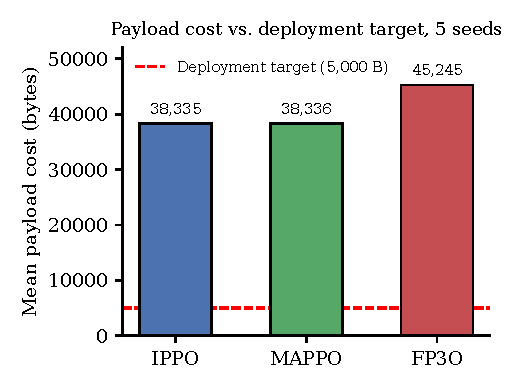
\includegraphics[width=0.85\linewidth]{figures/figure3_payload_safety_tradeoff.pdf}
\caption{Mean payload cost per algorithm (5 seeds), reconstructed from the project's leaderboard data, against the 5,000-byte deployment target. All three algorithms hold safety-shield activation at 0\% (omitted as a separate axis since it shows no dynamic range).}
\label{fig:payload}
\end{figure}
 
The S1--S4 progression narrows the design question from a binary ``is specialization necessary?'' to a sharper one: under what degree of functional heterogeneity does specialization become necessary for a fleet-wide OTA scheduler, given sufficiently informative type-conditioning, and does specialization introduce optimization-stability costs of its own? Our 5-seed result is directionally consistent with type-conditioned sharing matching or exceeding FP3O's specialized-head architecture with substantially lower cross-seed variance, but none of the pairwise comparisons are statistically significant at this sample size, so this should be read as suggestive rather than confirmatory evidence.
 
\section{Discussion and Limitations}
Several limitations qualify our conclusions for deployment purposes. First, although scaling from 2 to 5 seeds meaningfully tightened the IPPO/MAPPO estimates, we remain short of the 10 seeds originally planned, and the FP3O comparison in particular is underpowered ($p=0.285$, $d=0.78$) because a single outlier seed dominates its variance; the root cause of that seed's collapse (a late-training instability similar to those fixed during our training-stability work, versus a genuine bad optimum in one specialized head) has not yet been diagnosed. Second, TensorBoard logs were not retained for any run performed to date, so per-timestep training-curve and policy-entropy figures cannot be reconstructed for any past experiment, including the current headline run; this is a permanent gap in already-collected data rather than a pending regeneration step, and logging will be enabled prospectively. Third, mean payload cost for every algorithm remains 7--9$\times$ above the 5,000-byte deployment target, indicating that further reward or cost-shaping work is needed regardless of which architecture is chosen. Finally, all experiments use a synthetic cost model rather than real vehicle telemetry, network traces, or firmware images, which bounds the external validity of our specific numerical results, though not, we argue, the generality of the confound and instability findings themselves.
 
For a fleet-management system choosing between a shared or specialized OTA scheduler, our results suggest that a well-conditioned shared policy is both the more sample-efficient and the more reliable default under conflicting ECU-type incentives, provided the observation design is audited for identity leakage of the kind documented in Section~V -- a check we recommend for any MARL-based vehicular scheduler that reports a parameter-sharing result. Separately, FP3O's seed-instability finding suggests that specialized-head architectures may warrant explicit robustness testing across initializations before being considered for safety-relevant deployment, independent of their mean-case performance.
 
\section{Conclusion}
We studied whether a fleet-wide, safety-constrained automotive OTA update scheduler needs an explicitly specialized policy per ECU type, or whether a single, type-conditioned shared policy suffices. Using a staged experimental design scaled to 5 seeds per algorithm, we found that an apparently decisive early result favoring shared policies was driven by an agent-identity confound in the observation space, and that once corrected, the shared policy (IPPO/MAPPO) matches or exceeds the specialized architecture (FP3O) while being dramatically more stable across random seeds -- FP3O's headline mean is dominated by a single catastrophic-failure seed rather than uniformly weaker performance. The safety shield maintained a 0\% memory-safety violation rate throughout for all three algorithms. Future work will diagnose FP3O's failed seed, enable persistent training-diagnostic logging, scale to the originally planned 10 seeds per algorithm, close the remaining payload-cost gap to the deployment target, and evaluate the approach against real vehicle telemetry and larger, more diverse ECU fleets.
 
\section*{Code and Data Availability}
The environment, training code, and per-seed result files underlying this paper are publicly available at \url{https://github.com/saadmansakib47/Multiagent-ReLES-OTA}.
 
\section*{Acknowledgment}
The authors thank the Department of Computer Science and Engineering for providing the computational resources used in this work.
 
\begin{thebibliography}{00}
\bibitem{b1} A. Bhattacharjee, Z. Xu, V. Vyas, and W. Shi, ``ReLES-OTA: A reinforcement-learning enhanced scalable over-the-air update approach for CAVs,'' in \textit{2025 IEEE 3rd Int. Conf. Mobility, Operations, Services and Technologies (MOST)}, 2025, pp. 241--251.
\bibitem{b2} L. Feng, D. Xing, J. Zhang, and G. Pan, ``FP3O: Enabling proximal policy optimization in multi-agent cooperation with parameter-sharing versatility,'' 2023, arXiv:2310.05053.
\bibitem{b3} C. Yu, A. Velu, E. Vinitsky, J. Gao, Y. Wang, A. Bayen, and Y. Wu, ``The surprising effectiveness of PPO in cooperative multi-agent games,'' in \textit{Advances in Neural Information Processing Systems (NeurIPS), Datasets and Benchmarks Track}, 2022, arXiv:2103.01955.
\bibitem{b4} J. Schulman, F. Wolski, P. Dhariwal, A. Radford, and O. Klimov, ``Proximal policy optimization algorithms,'' 2017, arXiv:1707.06347.
\bibitem{b8} M. Towers, A. Kwiatkowski, J. Terry, J. U. Balis, G. De Cola, T. Deleu, M. Goul{\~a}o, A. Kallinteris, M. Krimmel, A. KG, R. Perez-Vicente, A. Pierr{\'e}, S. Schulhoff, J. J. Tai, H. Tan, and O. G. Younis, ``Gymnasium: A standard interface for reinforcement learning environments,'' 2024, arXiv:2407.17032.
\bibitem{b9} J. K. Terry, B. Black, N. Grammel, M. Jayakumar, A. Hari, R. Sullivan, L. S. Santos, C. Dieffendahl, C. Horsch, R. Perez-Vicente, N. Williams, Y. Lokesh, and P. Ravi, ``PettingZoo: Gym for multi-agent reinforcement learning,'' in \textit{Advances in Neural Information Processing Systems (NeurIPS), Datasets and Benchmarks Track}, vol. 34, 2021.
\bibitem{b10} R. Lowe, Y. Wu, A. Tamar, J. Harb, P. Abbeel, and I. Mordatch, ``Multi-agent actor-critic for mixed cooperative-competitive environments,'' in \textit{Advances in Neural Information Processing Systems (NeurIPS)}, vol. 30, 2017.
\bibitem{b11} J. Foerster, G. Farquhar, T. Afouras, N. Nardelli, and S. Whiteson, ``Counterfactual multi-agent policy gradients,'' in \textit{Proc. AAAI Conf. Artificial Intelligence}, vol. 32, no. 1, 2018.
\bibitem{b12} P. Sunehag, G. Lever, A. Gruslys, W. M. Czarnecki, V. Zambaldi, M. Jaderberg, M. Lanctot, N. Sonnerat, J. Z. Leibo, K. Tuyls, and T. Graepel, ``Value-decomposition networks for cooperative multi-agent learning based on team reward,'' in \textit{Proc. 17th Int. Conf. Autonomous Agents and MultiAgent Systems (AAMAS)}, 2018, pp. 2085--2087.
\bibitem{b13} T. Rashid, M. Samvelyan, C. Schroeder de Witt, G. Farquhar, J. Foerster, and S. Whiteson, ``QMIX: Monotonic value function factorisation for deep multi-agent reinforcement learning,'' in \textit{Proc. 35th Int. Conf. Machine Learning (ICML)}, 2018.
\bibitem{b14} J. K. Terry, N. Grammel, S. Son, B. Black, and A. Agrawal, ``Revisiting parameter sharing in multi-agent deep reinforcement learning,'' 2020, arXiv:2005.13625.
\bibitem{b15} A. D. Ames, S. Coogan, M. Egerstedt, G. Notomista, K. Sreenath, and P. Tabuada, ``Control barrier functions: Theory and applications,'' in \textit{2019 18th European Control Conf. (ECC)}, 2019, pp. 3420--3431.
\bibitem{b16} K. Smith \textit{et al.}, ``Robust and safe multi-agent reinforcement learning with communication for autonomous vehicles: From simulation to hardware,'' 2025, arXiv:2506.00982.
\bibitem{b17} Y. Guo, J. Liu, R. Yu, P. Hang, and J. Sun, ``MAPPO-PIS: A multi-agent proximal policy optimization method with prior intent sharing for CAVs' cooperative decision-making,'' in \textit{Computer Vision -- ECCV 2024 Workshops}, Lecture Notes in Computer Science, vol. 15630, Springer, 2025.
\bibitem{b18} L. S. Shapley, ``A value for n-person games,'' in \textit{Contributions to the Theory of Games II}, H. W. Kuhn and A. W. Tucker, Eds., Annals of Mathematics Studies, vol. 28. Princeton, NJ: Princeton Univ. Press, 1953, pp. 307--317.
\bibitem{b19} D. P. Kingma and J. Ba, ``Adam: A method for stochastic optimization,'' in \textit{Proc. 3rd Int. Conf. Learning Representations (ICLR)}, 2015.
\bibitem{b20} A. Raffin, A. Hill, A. Gleave, A. Kanervisto, M. Ernestus, and N. Dormann, ``Stable-Baselines3: Reliable reinforcement learning implementations,'' \textit{Journal of Machine Learning Research}, vol. 22, no. 268, pp. 1--8, 2021.
\end{thebibliography}
 
\end{document}
 